
%=================================================================
%                           Start Document
%=================================================================

\setstretch{1.6}
\sectiontitle{6}{Appendix}
\lhead{Appendix} % section header

\appendix
\lhead{Appendix A: Protocol for Running the Experimental Setup} % section header
\section{Protocol for Running the Experimental Setup}
\label{app:protocol}

This appendix outlines the step-by-step procedure required to run the Ribbit system, including initialization of the hardware and software components. This protocol ensures the correct startup and calibration of the robotic system and the real-time vision module.

\subsection*{Required Software and Hardware}
\begin{itemize}
    \item Qt Creator (to run the Ribbit GUI)
    \item Visual Studio (to run the 2D Vision real-time system)
    \item Brushless motor power supply (set to 12\,V)
    \item LED light source
\end{itemize}

\subsection*{Startup and Initialization Protocol}

\begin{enumerate}
    \item \textbf{Launch Qt Creator.} Open the Ribbit program.
    \item \textbf{Launch Visual Studio.} Open the \texttt{2D\_vision\_realtime} project.
    \item \textbf{Power on the system:}
    \begin{itemize}
        \item Turn on the 12\,V power supply for the brushless motors.
        \item Turn on the LED light source.
    \end{itemize}
    \item \textbf{Run the vision system:} Start the vision code from within Visual Studio.
    \item \textbf{Run the Qt GUI:} Compile and run the Ribbit program in Qt Creator.
\end{enumerate}

\subsection*{Initial PID Setup and Linear Stage Calibration}

\begin{enumerate}[resume]
    \item When the GUI opens, navigate to the \textbf{PID Controller} tab.
    \item If this is the first session of the day:
    \begin{enumerate}
        \item Set the four tendon tension setpoints to your desired initial values.
        \item Press \textbf{Start PID}.
        \item Press the \textbf{Reference} button to calibrate the linear stage.
        \item Wait for the referencing process to complete.
        \item Press \textbf{Stop PID}.
    \end{enumerate}
    \item Move the linear stage back by 2\,mm using the \textbf{Move to Position} function.
    \item Press the \textbf{Calibrate} button for each force sensor to zero the force readings.
\end{enumerate}

\subsection*{Final Setup for Operation}

\begin{enumerate}[resume]
    \item After sensor calibration, set the tendon tension setpoints to \textbf{100} for each channel.
    \item Press \textbf{Set} to confirm the new setpoints.
    \item Press \textbf{Start PID}.
    \item Go to the \textbf{Move to Position} field, enter \textbf{145\,mm}, and press \textbf{Move}.
    \item Wait for the linear stage to reach position. At this point, the tip should be exiting the robotic device and the system is ready for operation.
\end{enumerate}

\subsection*{Notes}
\begin{itemize}
    \item Always ensure the linear stage is referenced before moving to any absolute position.
    \item Force sensor calibration should be done only after referencing and initial positioning.
    \item Setpoint values can be adjusted depending on the specific experimental conditions.
\end{itemize}


\newpage
\lhead{Appendix B: Qt Control System Class Descriptions} % section header
\section{Qt Control System Class Descriptions}
\begin{longtable}{|>{\raggedright\arraybackslash}p{0.25\textwidth}|>{\raggedright\arraybackslash}p{0.7\textwidth}|}
\toprule
\textbf{Class Name} & \textbf{Description} \\
\midrule
\endfirsthead

\toprule
\textbf{Class Name} & \textbf{Description} \\
\midrule
\endhead

\bottomrule
\endfoot

\bottomrule
\endlastfoot

\rowcolor{folderblue}
\multicolumn{2}{|c|}{\textcolor{white}{\textbf{\large  Root Directory (Ribbot/)}}} \\
\midrule
\cellcolor{lightblue}\textbf{MainWindow} & Main GUI application window that coordinates all subsystems, handles user interactions, manages timers for sensor data acquisition, graph updates, and logging. Serves as the central hub connecting vision, motor control, and testing components. \\
\hline
\cellcolor{lightblue}\textbf{AirCalibrator} & Performs automated air calibration sequences by systematically varying tendon tensions while capturing vision data. Manages the calibration protocol including initial positioning, tension ramping, and data collection. \\
\hline
\cellcolor{lightblue}\textbf{Logger} & Handles comprehensive data logging to CSV files including force measurements, PID parameters, stage motion, vision data, and path following metrics. Manages threaded file I/O with queue-based buffering for real-time performance. \\
\hline
\cellcolor{lightblue}\textbf{Sensor} & Interfaces with force sensors for tendon tension measurement. Handles ADC conversion, sensor calibration/taring, and force unit conversion using the Sensoray 826 board. \\
\hline
\cellcolor{lightblue}\textbf{Tester} & Performs automated testing protocols for device characterization. Manages test sequences including initial insertion, tension application phases, and retraction while coordinating logging and vision recording. \\
\midrule

\rowcolor{folderblue}
\multicolumn{2}{|c|}{\textcolor{white}{\textbf{\large  Motor Control (motorcontrol/)}}} \\
\midrule
\cellcolor{lightblue}\textbf{LinearStageController} & Controls the PI linear stage for ribbon insertion and retraction. Manages positioning, speed control, acceleration/deceleration profiles, and provides motion status feedback via Qt signals. \\
\hline
\cellcolor{lightblue}\textbf{StageMotionEstimator} & Estimates real-time position and velocity of the linear stage based on motion profiles. Calculates acceleration, cruise, and deceleration phases for accurate motion prediction and timing. \\
\hline
\cellcolor{lightblue}\textbf{BrushlessMotor} & Controls individual brushless motors for tendon actuation. Manages motor voltage, direction, and velocity-to-voltage conversion using the Sensoray 826 DAQ board interface. \\
\hline
\cellcolor{lightblue}\textbf{initBoard} & Initializes and establishes connection to the Sensoray 826 DAQ board for hardware communication with sensors and actuators. \\
\midrule

\rowcolor{folderblue}
\multicolumn{2}{|c|}{\textcolor{white}{\textbf{\large  Tendon PID Control (tendonpids/)}}} \\
\midrule
\cellcolor{lightblue}\textbf{TendonPIDManager} & Coordinates PID control for all four tendon motors simultaneously. Manages setpoint ramping, synchronizes motor commands, and integrates linear stage feedforward compensation for consistent tension control. \\
\hline
\cellcolor{lightblue}\textbf{TendonPID} & Individual PID controller for each tendon with separate pull/release gains. Implements anti-windup, derivative filtering, and adaptive control based on stage motion state. \\
\midrule

\rowcolor{folderblue}
\multicolumn{2}{|c|}{\textcolor{white}{\textbf{\large Vision System (vision/)}}} \\
\midrule
\cellcolor{lightblue}\textbf{VisionReceiver} & Receives 3D vision data (tip position, pre-tip position, direction vector) from Python vision system via ZeroMQ. Validates data integrity and emits Qt signals for real-time feedback. \\
\hline
\cellcolor{lightblue}\textbf{VisionSender} & Sends commands to the vision system for video recording control and frame capture during calibration sequences. Uses ZeroMQ for reliable communication with Python vision interface. \\
\midrule

\rowcolor{folderblue}
\multicolumn{2}{|c|}{\textcolor{white}{\textbf{\large  Path Following (pathfollowing/)}}} \\
\midrule
\cellcolor{lightblue}\textbf{PathFollower} & Implements closed-loop path following control combining feedforward and feedback components. Orchestrates vision-based guidance, curvature control, and tendon tension commands for trajectory tracking. \\
\hline
\cellcolor{lightblue}\textbf{FeedbackController} & PID controller for path following that converts pitch angle errors to curvature commands. Features asymmetric gains for left/right steering and integral anti-windup mechanisms. \\
\hline
\cellcolor{lightblue}\textbf{LineOfSight} & Computes line-of-sight guidance angles and waypoint tracking for path following. Calculates cross-track error and reference heading angles based on current position and desired trajectory. \\
\hline
\cellcolor{lightblue}\textbf{PathProcessing} & Processes CSV path files containing curvature and length data to generate discrete waypoints for trajectory following. Handles both straight and curved path segments with configurable step sizes. \\
\hline
\cellcolor{lightblue}\textbf{PitchConverter} & Converts 3D direction vectors from vision system to pitch angles for steering control. Includes smoothing filters to reduce noise in angle measurements. \\
\hline
\cellcolor{lightblue}\textbf{RibbonAdapter} & Adapts generic curvature commands to ribbon-specific actuation parameters. Implements calibrated mapping between desired curvature and required tendon tension differences. \\
\hline
\cellcolor{lightblue}\textbf{TensionConverter} & Converts differential actuation commands to individual tendon tension setpoints. Ensures minimum tension levels and handles tension limits for safe operation. \\
\hline
\cellcolor{lightblue}\textbf{FeedforwardCalculator} & Calculates feedforward control signals based on path curvature to improve tracking performance. Generates tension commands that anticipate required steering forces along the trajectory. \\

\end{longtable}
\newpage


\lhead{Appendix C: Vision System Class Descriptions} % section header
\section{Vision System Class Descriptions}
\begin{longtable}{|>{\raggedright\arraybackslash}p{0.25\textwidth}|>{\raggedright\arraybackslash}p{0.7\textwidth}|}
\toprule
\textbf{Class Name} & \textbf{Description} \\
\midrule
\endfirsthead

\toprule
\textbf{Class Name} & \textbf{Description} \\
\midrule
\endhead

\bottomrule
\endfoot

\bottomrule
\endlastfoot

\rowcolor{folderblue}
\multicolumn{2}{|c|}{\textcolor{white}{\textbf{\large  Core Vision System}}} \\
\midrule
\cellcolor{lightblue}\textbf{CameraSystem} & Manages dual Basler camera interface using PyPylon library. Handles camera configuration including exposure settings and frame rate control. Implements threaded frame acquisition with latest-frame-only strategy and provides synchronized stereo image pairs through a thread-safe queue system. \\
\hline
\cellcolor{lightblue}\textbf{ObjectDetector} & Core detection engine that processes stereo camera frames to identify catheter tip and orientation. Uses background subtraction, morphological operations, and skeleton-based analysis to extract tip position, pre-tip reference point, and direction vector. Implements threaded processing for real-time performance. \\
\hline
\cellcolor{lightblue}\textbf{Undistorter} & Handles camera calibration and image rectification using stored calibration parameters. Performs lens distortion correction, maintains adaptive reference frame through temporal averaging, and manages coordinate transformations between camera and world coordinate systems. \\
\midrule

\rowcolor{folderblue}
\multicolumn{2}{|c|}{\textcolor{white}{\textbf{\large  Communication \& Control}}} \\
\midrule
\cellcolor{lightblue}\textbf{Communicator} & Manages bidirectional ZeroMQ communication with the Qt control system. Publishes real-time 3D position and orientation data via PUB socket, receives control commands via ROUTER socket, and handles coordinate system transformations from pixels to millimeters for control system integration. \\
\midrule

\rowcolor{folderblue}
\multicolumn{2}{|c|}{\textcolor{white}{\textbf{\large  Data Recording \& Visualization}}} \\
\midrule
\cellcolor{lightblue}\textbf{Recorder} & Recording system for experimental data capture. Manages synchronized dual-camera video recording, handles on-demand frame capture for calibration sequences, organizes data into timestamped session folders, and provides MP4 video output with configurable compression settings. \\
\hline
\cellcolor{lightblue}\textbf{Visualizer} & Real-time visualization system for system monitoring and debugging. Displays live camera feeds, overlays detection results including tip position and orientation arrows, provides side-by-side comparison views, and manages OpenCV window operations for user interface. \\

\end{longtable}

\lhead{Appendix D: Vision System Sequence Diagrams} % section header
\section{Vision System Sequence Diagrams}
\begin{figure} [H]
    \centering
    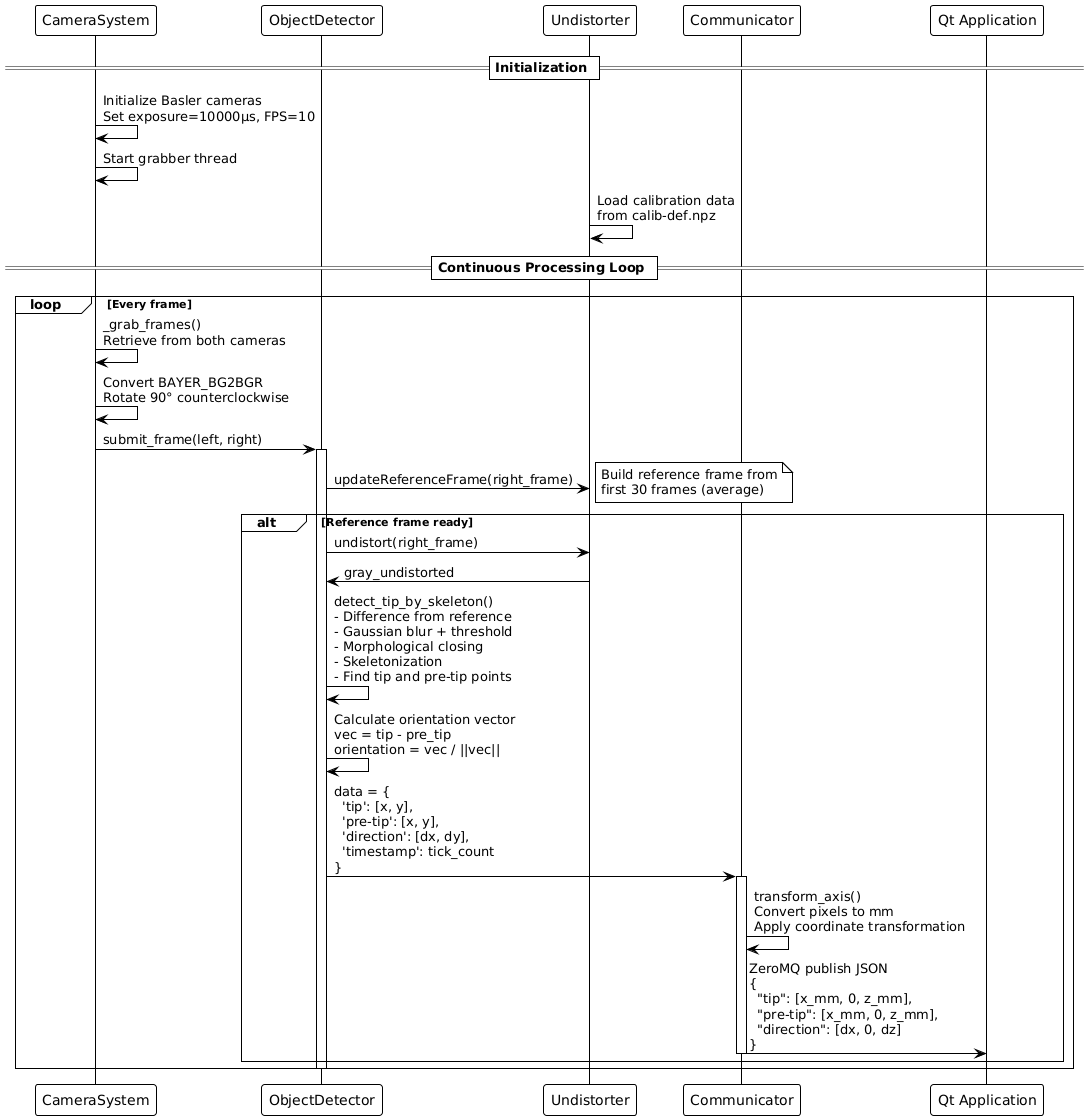
\includegraphics[width=1.1\linewidth]{images/vision/pythonSequencediag.png}
    \caption{Sequence diagram of Python Tip detection code}
    \label{fig:seqpython}
\end{figure}
\newpage

\lhead{Appendix E: Vision System Sequence Diagram} % section header
\section{Tip Tracking Integration Theory: Types of Communication Protocols}

There are several ways to establish a communication layer that allows real-time data transfer between two programs, often referred to as InterProcess Communication (IPC). Below is a brief analysis of each relevant method.

\begin{figure} [H]
    \centering
    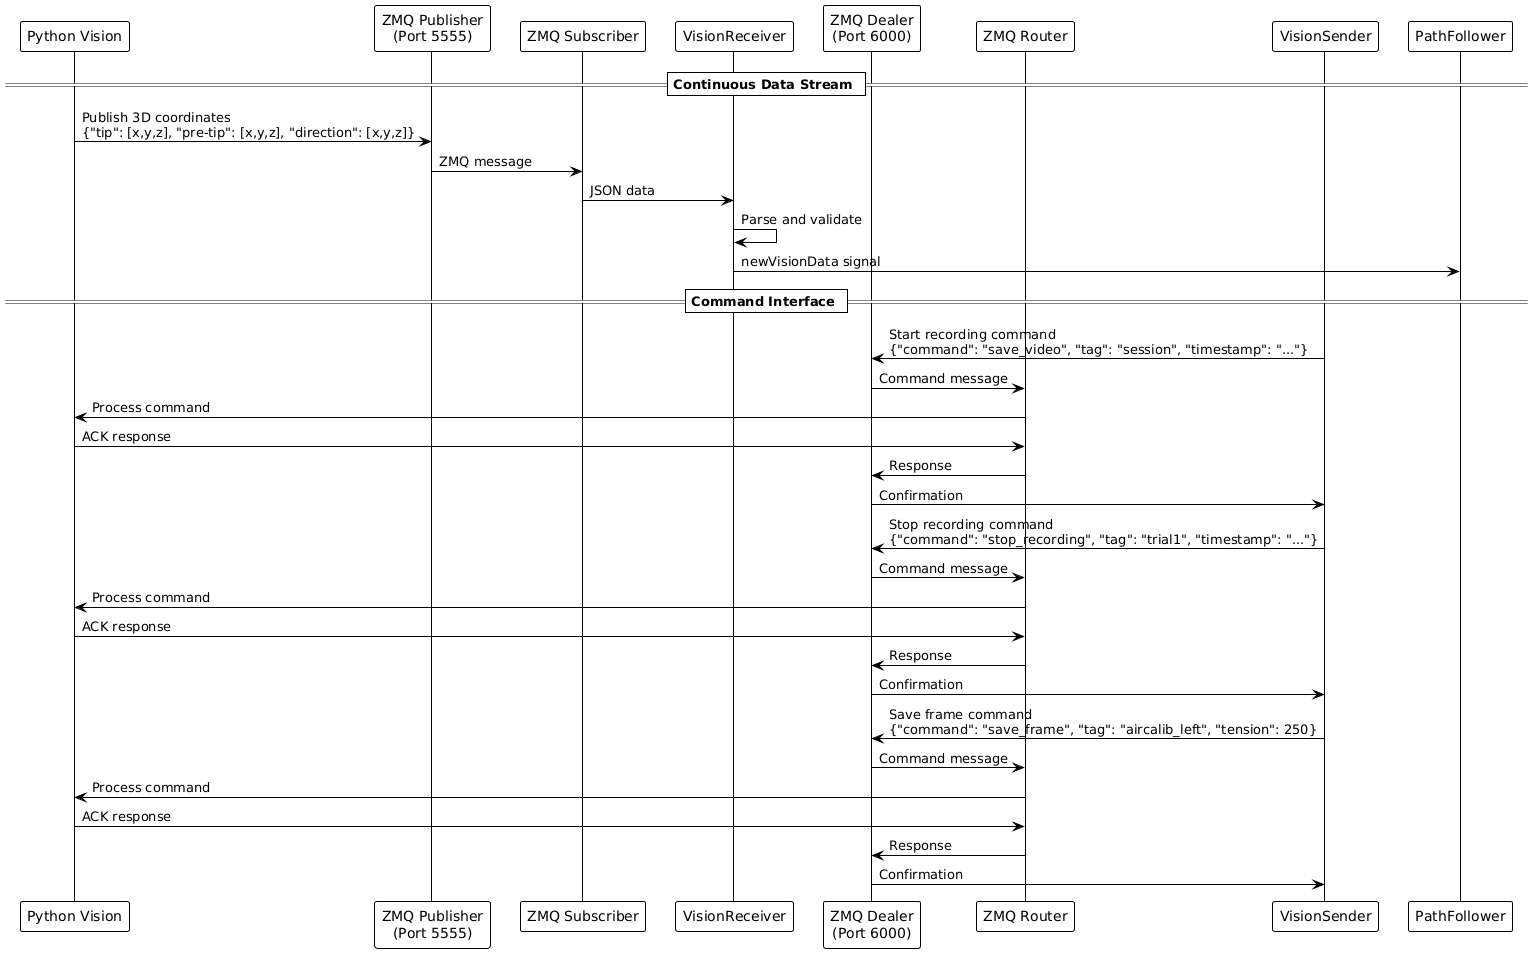
\includegraphics[width=1.1\linewidth]{images/Software documentation/visionSequencediag.png}
    \caption{Sequence diagram of the communication between python vision system and Qt control system}
    \label{fig:seqComm}
\end{figure}


\paragraph*{File-based communication}
The simplest solution in terms of implementation is file based communication. One system would for each data point write to a file which is subsequently read by the receiving system. This requires the receiving system to continuously monitor the file for updates introducing latency that is further exacerbated by file system access times and disk I/O overhead. 

In terms of fault tolerance, file-based communication has the benefit of data persisting even if a process crashes, however it is not designed for high-frequency updates \cite{gray_interprocess_2003}. Race conditions can occur if both the vision and control systems attempt to access the file simultaneously. Locking mechanisms can mitigate this, but at the cost of further increasing latency \cite{gray_interprocess_2003}. 

\paragraph*{Shared memory}
A significantly faster method is shared memory. Shared memory allows multiple processes to access a common memory space, enables rapid data exchange without the overhead of disk I/O or network communication. However it also introduces concurrency and data consistency challenges. \cite{gray_interprocess_2003}

Since multiple processes may attempt to read and write simultaneously, synchronization mechanisms such as mutexes or semaphores are required to prevent race conditions \cite{burns_real-time_2009}. This adds complexity and thus makes the system less robust and maintainable. Another challenge is that shared memory must be allocated and managed by both processes. This makes it difficult to integrate across different programming languages where data structures may not be inherently compatible. Thus the complexity, lack of language compatibility and make it impractical for this application.

\paragraph*{Named Pipes}
Named Pipes allow data to be transmitted between processes on the same machine asynchronously by operating as a first-in, first-out (FIFO) buffer \cite{gray_interprocess_2003}. Compared to file-based communication, pipes offer lower latency and are more efficient for continuous data streaming \cite{gray_interprocess_2003}. The main limitation in the context of this project is that they are constrained to a single machine. This limits the scalability since in a later revision one might want to run the vision and control systems on separate machines in a distributed setup. 

\paragraph*{Message queues}
Message queues provide structured message passing using a queue-based architecture \cite{kleppmann_designing_2017}. Systems such as RabbitMQ and Apache Kafka provide reliable message delivery making message queues highly fault tolerant. However they also introduce latency due to message buffering and broker management \cite{kleppmann_designing_2017}. Meaning that they may not be ideal for real-time application such as this onw where low-latency streaming is of a higher priority than durable message queueing.

\paragraph*{Networking (Sockets and ZeroMQ)}
Networking-based communication, using either raw sockets or messaging libraries such as ZeroMQ \cite{noauthor_zeromq_nodate}, provides a flexible and scalable solution \cite{lauener_how_2018}. Raw sockets allow direct communication over a network using protocols such as TCP or UDP. TCP ensures reliable message delivery but introduces additional latency. The choice between TCP and UDP is a trade-off between reliability and variability of delays: UDP does not perform flow control and does not retransmit lost packets, so it avoids some of the resasons for variable network delays \cite{kleppmann_designing_2017}. Unlike TCP, UDP does not guarantee message delivery, meaning that packets may be lost.  However, for real-time control, receiving the most recent data is more important than ensuring that every packet arrives. Since the vision data is used as feedback, occasional packet loss is preferable to the latency caused by TCP retransmissions. 

ZeroMQ provides a higher-level abstraction for message-based communication and offers built-in support for various messaging patterns, including publish/subscribe (pub/sub), request/reply and push/pull \cite{lauener_how_2018}. The pub/sub model is especially advantageous system since it enables efficient real-time streaming of data to multiple subscribers with minimal overhead. 


%=================================================================
%                           End Document
%=================================================================
